\documentclass{standalone}

\usepackage{tikz}
\tikzset{>=stealth}
\usepackage{xcolor}
\usepackage{amsmath}


\begin{document}
    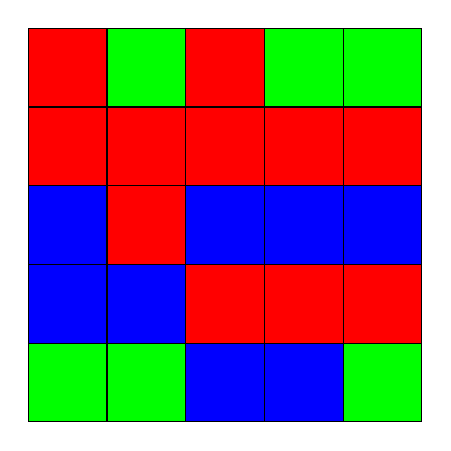
\begin{tikzpicture}
        \def\sqd{1}
    
        \draw[ fill=green] (0,0) rectangle (0+\sqd,0+\sqd);
        \draw[ fill=green] (1,0) rectangle (1+\sqd,0+\sqd);
        \draw[ fill=blue] (2,0) rectangle (2+\sqd,0+\sqd);
        \draw[ fill=blue] (3,0) rectangle (3+\sqd,0+\sqd);
        \draw[ fill=green] (4,0) rectangle (4+\sqd,0+\sqd);

        
        \draw[ fill=blue] (0,1) rectangle (0+\sqd,1+\sqd);
        \draw[ fill=blue] (1,1) rectangle (1+\sqd,1+\sqd);
        \draw[ fill=red] (2,1) rectangle (2+\sqd,1+\sqd);
        \draw[ fill=red] (3,1) rectangle (3+\sqd,1+\sqd);
        \draw[ fill=red] (4,1) rectangle (4+\sqd,1+\sqd);
        
        \draw[ fill=blue] (0,2) rectangle (0+\sqd,2+\sqd);
        \draw[ fill=red ] (1,2) rectangle (1+\sqd,2+\sqd);
        \draw[ fill=blue] (2,2) rectangle (2+\sqd,2+\sqd);
        \draw[ fill=blue] (3,2) rectangle (3+\sqd,2+\sqd);
        \draw[ fill=blue] (4,2) rectangle (4+\sqd,2+\sqd);


        \draw[fill=red] (0,3) rectangle (0+\sqd,3+\sqd);
        \draw[fill=red] (1,3) rectangle (1+\sqd,3+\sqd);
        \draw[fill=red] (2,3) rectangle (2+\sqd,3+\sqd);
        \draw[fill=red] (3,3) rectangle (3+\sqd,3+\sqd);
        \draw[fill=red] (4,3) rectangle (4+\sqd,3+\sqd);
        
        
        \draw[fill=red] (0,4) rectangle (0+\sqd,4+\sqd);
        \draw[fill=green] (1,4) rectangle (1+\sqd,4+\sqd);
        \draw[fill=red] (2,4) rectangle (2+\sqd,4+\sqd);
        \draw[fill=green] (3,4) rectangle (3+\sqd,4+\sqd);
        \draw[fill=green] (4,4) rectangle (4+\sqd,4+\sqd);

        %labels 
        % \draw[fill=black] (0,-3) circle (\radi) node {\textcolor{white}{$\beta$}}; 
        % \draw[fill=black] (0,3) circle (\radi) node {\textcolor{white}{$\alpha$}};
        % %pixels 
        % \draw[color=black] (-\sqpos-\squ,0-\squ) rectangle node{p} (-\sqpos+\squ,0+\squ);
        % \draw[fill=white] (\sqpos-\squ,0-\squ) rectangle node{q} (\sqpos+\squ,0+\squ);

        
    \end{tikzpicture}
\end{document}
